
\documentclass[letterpaper,hide notes,xcolor={table,svgnames},pdftex,10pt]{beamer}
\def\showexamples{t}


%\usepackage[svgnames]{xcolor}

%% Demo talk
%\documentclass[letterpaper,notes=show]{beamer}

\usecolortheme{crane}
\setbeamertemplate{navigation symbols}{}

\usetheme{MyPittsburgh}
%\usetheme{Frankfurt}

%\usepackage{tipa}

\usepackage{hyperref}
\usepackage{graphicx,xspace}
\usepackage[normalem]{ulem}
\usepackage{multicol}

\newcommand\SF[1]{$\bigstar$\footnote{SF: #1}}

\usepackage[default]{sourcesanspro}
\usepackage[T1]{fontenc}

\newcounter{tmpnumSlide}
\newcounter{tmpnumNote}

% old question code
%\newcommand\question[1]{{$\bigstar$ \small \onlySlide{2}{#1}}}
% \newcommand\nquestion[1]{\ifdefined \presentationonly \textcircled{?} \fi \note{\par{\Large \textbf{?}} #1}}
% \newcommand\nanswer[1]{\note{\par{\Large \textbf{A}} #1}}


 \newcommand\mnote[1]{%
   \addtocounter{tmpnumSlide}{1}
   \ifdefined\showcues {~\tiny\fbox{\arabic{tmpnumSlide}}}\fi
   \note{\setlength{\parskip}{1ex}\addtocounter{tmpnumNote}{1}\textbf{\Large \arabic{tmpnumNote}:} {#1\par}}}

\newcommand\mmnote[1]{\note{\setlength{\parskip}{1ex}#1\par}}

%\newcommand\mnote[2][]{\ifdefined\handoutwithnotes {~\tiny\fbox{#1}}\fi
% \note{\setlength{\parskip}{1ex}\textbf{\Large #1:} #2\par}}

%\newcommand\mnote[2][]{{\tiny\fbox{#1}} \note{\setlength{\parskip}{1ex}\textbf{\Large #1:} #2\par}}

\newcommand\mquestion[2]{{~\color{red}\fbox{?}}\note{\setlength{\parskip}{1ex}\par{\Large \textbf{?}} #1} \note{\setlength{\parskip}{1ex}\par{\Large \textbf{A}} #2\par}\ifdefined \presentationonly \pause \fi}

\newcommand\blackboard[1]{%
\ifdefined   \showblackboard
  {#1}
  \else {\begin{center} \fbox{\colorbox{blue!30}{%
         \begin{minipage}{.95\linewidth}%
           \hspace{\stretch{1}} Some space intentionally left blank; done at the blackboard.%
         \end{minipage}}}\end{center}}%
         \fi%
}



%\newcommand\q{\tikz \node[thick,color=black,shape=circle]{?};}
%\newcommand\q{\ifdefined \presentationonly \textcircled{?} \fi}

\usepackage{listings}
\lstset{%
  keywordstyle=\bfseries,
  aboveskip=15pt,
  belowskip=15pt,
  captionpos=b,
  identifierstyle=\ttfamily,
  escapeinside={(*@}{@*)},
  stringstyle=\ttfamiliy,
  frame=lines,
  numbers=left, basicstyle=\scriptsize, numberstyle=\tiny, stepnumber=0, numbersep=2pt}

\usepackage{siunitx}
\newcommand\sius[1]{\num[group-separator = {,}]{#1}\si{\micro\second}}
\newcommand\sims[1]{\num[group-separator = {,}]{#1}\si{\milli\second}}
\newcommand\sins[1]{\num[group-separator = {,}]{#1}\si{\nano\second}}
\sisetup{group-separator = {,}, group-digits = true}

%% -------------------- tikz --------------------
\usepackage{tikz}
\usetikzlibrary{positioning}
\usetikzlibrary{arrows,backgrounds,automata,decorations.shapes,decorations.pathmorphing,decorations.markings,decorations.text}

\tikzstyle{place}=[circle,draw=blue!50,fill=blue!20,thick, inner sep=0pt,minimum size=6mm]
\tikzstyle{transition}=[rectangle,draw=black!50,fill=black!20,thick, inner sep=0pt,minimum size=4mm]

\tikzstyle{block}=[rectangle,draw=black, thick, inner sep=5pt]
\tikzstyle{bullet}=[circle,draw=black, fill=black, thin, inner sep=2pt]

\tikzstyle{pre}=[<-,shorten <=1pt,>=stealth',semithick]
\tikzstyle{post}=[->,shorten >=1pt,>=stealth',semithick]
\tikzstyle{bi}=[<->,shorten >=1pt,shorten <=1pt, >=stealth',semithick]

\tikzstyle{mut}=[-,>=stealth',semithick]

\tikzstyle{treereset}=[dashed,->, shorten >=1pt,>=stealth',thin]

\usepackage{ifmtarg}
\usepackage{xifthen}
\makeatletter
% new counter to now which frame it is within the sequence
\newcounter{multiframecounter}
% initialize buffer for previously used frame title
\gdef\lastframetitle{\textit{undefined}}
% new environment for a multi-frame
\newenvironment{multiframe}[1][]{%
\ifthenelse{\isempty{#1}}{%
% if no frame title was set via optional parameter,
% only increase sequence counter by 1
\addtocounter{multiframecounter}{1}%
}{%
% new frame title has been provided, thus
% reset sequence counter to 1 and buffer frame title for later use
\setcounter{multiframecounter}{1}%
\gdef\lastframetitle{#1}%
}%
% start conventional frame environment and
% automatically set frame title followed by sequence counter
\begin{frame}%
\frametitle{\lastframetitle~{\normalfont(\arabic{multiframecounter})}}%
}{%
\end{frame}%
}
\makeatother

\makeatletter
\newdimen\tu@tmpa%
\newdimen\ydiffl%
\newdimen\xdiffl%
\newcommand\ydiff[2]{%
    \coordinate (tmpnamea) at (#1);%
    \coordinate (tmpnameb) at (#2);%
    \pgfextracty{\tu@tmpa}{\pgfpointanchor{tmpnamea}{center}}%
    \pgfextracty{\ydiffl}{\pgfpointanchor{tmpnameb}{center}}%
    \advance\ydiffl by -\tu@tmpa%
}
\newcommand\xdiff[2]{%
    \coordinate (tmpnamea) at (#1);%
    \coordinate (tmpnameb) at (#2);%
    \pgfextractx{\tu@tmpa}{\pgfpointanchor{tmpnamea}{center}}%
    \pgfextractx{\xdiffl}{\pgfpointanchor{tmpnameb}{center}}%
    \advance\xdiffl by -\tu@tmpa%
}
\makeatother
\newcommand{\copyrightbox}[3][r]{%
\begin{tikzpicture}%
\node[inner sep=0pt,minimum size=2em](ciimage){#2};
\usefont{OT1}{phv}{n}{n}\fontsize{4}{4}\selectfont
\ydiff{ciimage.south}{ciimage.north}
\xdiff{ciimage.west}{ciimage.east}
\ifthenelse{\equal{#1}{r}}{%
\node[inner sep=0pt,right=1ex of ciimage.south east,anchor=north west,rotate=90]%
{\raggedleft\color{black!50}\parbox{\the\ydiffl}{\raggedright{}#3}};%
}{%
\ifthenelse{\equal{#1}{l}}{%
\node[inner sep=0pt,right=1ex of ciimage.south west,anchor=south west,rotate=90]%
{\raggedleft\color{black!50}\parbox{\the\ydiffl}{\raggedright{}#3}};%
}{%
\node[inner sep=0pt,below=1ex of ciimage.south west,anchor=north west]%
{\raggedleft\color{black!50}\parbox{\the\xdiffl}{\raggedright{}#3}};%
}
}
\end{tikzpicture}
}


%% --------------------

%\usepackage[excludeor]{everyhook}
%\PushPreHook{par}{\setbox0=\lastbox\llap{MUH}}\box0}

%\vspace*{\stretch{1}

%\setbox0=\lastbox \llap{\textbullet\enskip}\box0}

\setlength{\parskip}{\fill}

\newcommand\noskips{\setlength{\parskip}{1ex}}
\newcommand\doskips{\setlength{\parskip}{\fill}}

\newcommand\xx{\par\vspace*{\stretch{1}}\par}
\newcommand\xxs{\par\vspace*{2ex}\par}
\newcommand\tuple[1]{\langle #1 \rangle}
\newcommand\code[1]{{\sf \footnotesize #1}}
\newcommand\ex[1]{\uline{Example:} \ifdefined \presentationonly \pause \fi
  \ifdefined\showexamples#1\xspace\else{\uline{\hspace*{2cm}}}\fi}

\newcommand\ceil[1]{\lceil #1 \rceil}


\AtBeginSection[]
{
   \begin{frame}
       \frametitle{Outline}
       \tableofcontents[currentsection]
   \end{frame}
}



\pgfdeclarelayer{edgelayer}
\pgfdeclarelayer{nodelayer}
\pgfsetlayers{edgelayer,nodelayer,main}

\tikzstyle{none}=[inner sep=0pt]
\tikzstyle{rn}=[circle,fill=Red,draw=Black,line width=0.8 pt]
\tikzstyle{gn}=[circle,fill=Lime,draw=Black,line width=0.8 pt]
\tikzstyle{yn}=[circle,fill=Yellow,draw=Black,line width=0.8 pt]
\tikzstyle{empty}=[circle,fill=White,draw=Black]
\tikzstyle{bw} = [rectangle, draw, fill=blue!20, 
    text width=4em, text centered, rounded corners, minimum height=2em]
    
    \newcommand{\CcNote}[1]{% longname
	This work is licensed under the \textit{Creative Commons #1 3.0 License}.%
}
\newcommand{\CcImageBy}[1]{%
	\includegraphics[scale=#1]{creative_commons/cc_by_30.pdf}%
}
\newcommand{\CcImageSa}[1]{%
	\includegraphics[scale=#1]{creative_commons/cc_sa_30.pdf}%
}
\newcommand{\CcImageNc}[1]{%
	\includegraphics[scale=#1]{creative_commons/cc_nc_30.pdf}%
}
\newcommand{\CcGroupBySa}[2]{% zoom, gap
	\CcImageBy{#1}\hspace*{#2}\CcImageNc{#1}\hspace*{#2}\CcImageSa{#1}%
}
\newcommand{\CcLongnameByNcSa}{Attribution-NonCommercial-ShareAlike}

\newenvironment{changemargin}[1]{% 
  \begin{list}{}{% 
    \setlength{\topsep}{0pt}% 
    \setlength{\leftmargin}{#1}% 
    \setlength{\rightmargin}{1em}
    \setlength{\listparindent}{\parindent}% 
    \setlength{\itemindent}{\parindent}% 
    \setlength{\parsep}{\parskip}% 
  }% 
  \item[]}{\end{list}} 




\title{Lecture 28 --- Case Study: Bre-X }

\author{Jeff Zarnett, based on original by Douglas Harder \\ \small \texttt{jzarnett@uwaterloo.ca} / \texttt{dwharder@uwaterloo.ca}}
\institute{Department of Electrical and Computer Engineering \\
  University of Waterloo}
\date{\today}


\begin{document}

\begin{frame}
  \titlepage

\begin{center}
  \small{Acknowledgments: Douglas Harder~\cite{dwh}, Julie Vale~\cite{jv}}
  \end{center}
\end{frame}



\begin{frame}
\frametitle{Bre-X}

In 1993, Bre-X was a penny-stock mining company with stocks selling at \$0.27.

David Walsh (owner) wished to buy a gold claim in Busang, Indonesia.

The highlands were formed by a massive volcano.

Numerous Australian companies had already prospected the island.\\
\quad They were only able to establish a single viable mine.

The Grasberg Gold Mine in New Guinea is the largest in the world.

\end{frame}



\begin{frame}
\frametitle{Busang, Indonesia}

\begin{center}
	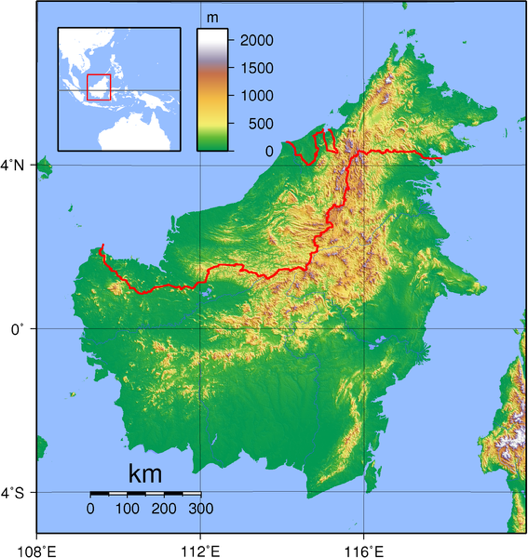
\includegraphics[width=0.5\textwidth]{images/busang.png}
\end{center}

\end{frame}



\begin{frame}
\frametitle{Bre-X}

David Walsh was wined and dined by two geologists: John Felderhof \& Michael de Guzman.

Walsh committed \$80,000 to the Busang project.

De Guzman was an engineer with a colourful character:
\begin{itemize}
	\item At the top of his class
	\item As a Filipino, he was, however, subject to a low glass ceiling
	\item  He had four wives with families, simultaneously, all of whom were unaware of each other
\end{itemize}

\end{frame}



\begin{frame}
\frametitle{1994}

First they had to ``partner'' with an Indonesian.\\
\quad They found Sigit Hardjojudanto, Suharto's son.

They began to find gold...\\
\quad Early 1994:		  2 million oz\\
\quad Mid 1994:		  3 million oz\\
\quad Late 1994:		  8 million oz

Stocks were trading at \$2.05

Yes, gold is measured in ounces, despite it being a non-metric unit...\\
\quad 1 Troy Ounce is 31.1035g.

\end{frame}



\begin{frame}
\frametitle{1995}

1995 continued to be a good year; the stock price was \$14.87 by the end of July.

The reserves only increased:\\
\quad 1995:			10 million oz\\
\quad Speculation:		30 million oz

The stock was now at \$50 per share!

\end{frame}



\begin{frame}
\frametitle{1996}

Normal practice is to store half of a core sample for verification.

De Guzman was crushing the entire core claiming the ``nugget effect''.

That is, the inability to get a statistically valid sample for analysis.\\
\quad The theory is that gold is not evenly distributed throughout the sample.

\end{frame}



\begin{frame}
\frametitle{1996}

An auditor noted that the gold in the samples were rounded -- more like alluvial gold.

Alluvial gold is found in alluvium: clay, sand, gravel, or similar material deposited by running water (according to Merriam-Webster Dictionary).


De Guzman gave a volcanic pool theory accounted the rounded corners of the gold found in the core samples.


\end{frame}



\begin{frame}
\frametitle{1996}

Bre-X is now traded on the Toronto Stock Exchange (then, TSE, now TSX):\\
\quad April:				\$180\\
\quad Early May:		\$200\\
\quad Late May:		\$286.50

New announcements:\\
\quad June:			39 million oz\\
\quad Early July:	42.6 million oz\\
\quad Late July:	47 million oz

Numerous mining companies -- mostly Canadian -- were headed off to Borneo staking other claims...


Felderhof sold \$84 million worth of stocks.


\end{frame}



\begin{frame}
\frametitle{1996}

At this time, Trevor Cavicchi was Canadian geologist who had just graduated from university.

	He was hired by Bre-X and, in Borneo, had noted
numerous core samples lying open.

This is something that would not be considered among best practices.

He asked a few questions but was quickly told off.

As a junior geologist, he didn't pursue the issue...

\end{frame}



\begin{frame}
\frametitle{The Wrong Kind of Attention}

Now, Bre-X was attracting the attention of the Indonesian strongman Suharto.

Indonesia revoked Bre-X's explorations rights claiming irregularities.

Freeport McMoRan Copper \& Gold Inc. was brought in by Indonesia to exploit the mine.

A company employing one of Suharto's daughters would be building the infrastructure.

Following a resolution to a 10-month dispute:\\
\quad Bre-X						45\%
\quad Freeport					15\%
\quad The Indonesian government	40\%

\end{frame}



\begin{frame}
\frametitle{1997}

Bre-X's stock was dropping:  to prop it up, they ``found'' more gold.\\
\quad February 17:			71 million oz\\
\quad February 19:			Claims of 200 million oz

The stock prices recovered and Felderhof is awarded the ``Man of the Year Award'' from the Prospectors \& Developers Association of Canada.

De Guzman's office at Busang is destroyed by fire...

\end{frame}



\begin{frame}
\frametitle{Do Your Own Homework}

Unfortunately, Freeport was digging its own cores.

They dug a sample only 1.5 m away from Bre-X site.

Their core found 0.01 grams per tonne.

Bre-X had found 4.39 grams per tonne.

\end{frame}



\begin{frame}
\frametitle{The End of De Guzman}

De Guzman was in Toronto addressing shareholders but is called back to explain the discrepancy in Freeport's findings.

During the helicopter flight, he appears to have jumped into the Indonesian jungle, committing suicide (allegedly).

Rumours continue to this day about whether he was pushed...

What appears to be his body, badly decomposed, was found four days later.

\end{frame}



\begin{frame}
\frametitle{It All Comes Crashing Down}

The stock price of Bre-X dropped to almost nothing...
\begin{itemize}
\item All involved blamed everything on de Guzman
\item Walsh moves to the Bahamas
\item Felderhof moves to the Cayman Islands
\item No one is found guilty of this fraud
\item Joe Groia, who successfully defended Felderhoff, was found guilty of professional misconduct in June 2012 by the Law Society of Upper Canada for his conduct during the trial
\end{itemize}


\end{frame}



\begin{frame}
\frametitle{A Little Salt, Hold the Pepper}

De Guzman had been salting the core samples.

He used gold from one of his wedding bands.

Initially, it was 3 oz per tonne -- a modest amount, but this rose over the years.

Later, de Guzman ended up purchasing \$61,000 of alluvial gold

He was very intelligent in measuring plausible quantities of gold into each sample -- never more than could have been believable given the current hype.

\end{frame}



\begin{frame}
\frametitle{We Blew It}

The Canadian mining industry was seen as the laughing stock of the world.

Prior to this, the industry was not regulated.

Regulation similar to that of engineering was introduced.

\end{frame}



\begin{frame}
\frametitle{Geoscience}

In Ontario, the Professional Geoscientists Act was passed in 2000.

Geosciences would now be a self-regulating profession.

Modeled on the Professional Engineers Act.

The Act established the Association of Professional Geoscientists of Ontario (APGO).

After a 3-year transitional council, the first elected council was formed in 2003.

Students graduating from geological engineering at UW satisfy the requirements of both PEO and the APGO.

\end{frame}



\begin{frame}
\frametitle{Response}

In Alberta, the professions of engineering and geoscience form one association.

One silver lining: Trevor Cavicchi has since gone on to become a successful geologist.

He has apparently gained a reputation for stating the facts and not attempting to manipulate them to satisfy the wants or desires of others.

\end{frame}



\begin{frame}
\frametitle{References \& Disclaimer}
\bibliographystyle{alphaurl}
\setbeamertemplate{bibliography item}{\insertbiblabel}
{\scriptsize
\bibliography{290}
}
\vfill

{\tiny Disclaimer: the material presented in these lectures slides is intended for use in the course ECE~290 at the University of Waterloo and should not be relied upon as legal advice. Any reliance on these course slides by any party for any other purpose are the responsibility of such parties.  The author(s) accept(s) no responsibility for damages, if any, suffered by any party as a result of decisions made or actions based on these course slides for any other purpose than that for which it was intended.\par}


\end{frame}


\end{document}

